\documentclass[a4paper, 12pt]{article}
% page
% \usepackage[top=2.54cm,bottom=2.54cm,left=3.18cm,right=3.18cm]{geometry}  % default
\usepackage{graphicx}
\usepackage[top=2.27cm,bottom=1.27cm,left=1.27cm,right=1.27cm]{geometry}
% \usepackage[none]{hyphenat} % remove hyphen
\usepackage[hidelinks]{hyperref}    % remove hyperref box

% header and footer
\usepackage{fancyhdr}
\fancypagestyle{plain}{
    \fancyhead[L]{}
    \fancyhead[C]{Computer Vision HW3 Report}
    \fancyhead[R]{Student ID: R11625015\\ Name: 廖致豪}
    % \fancyfoot[L]{}
    % \fancyfoot[C]{}
    % \fancyfoot[R]{}
    \renewcommand{\headrulewidth}{0.5pt}
    \renewcommand{\footrulewidth}{0pt}
    % \setlength{\headheight}{}
    % \addtolength{\topmargin}{}
}
\pagestyle{plain}

% font setting
\usepackage{fontspec}
\usepackage{xeCJK}
    \setCJKmainfont{標楷體}
    % \setCJKmainfont{微軟正黑體}
    \XeTeXlinebreaklocale "zh"
    \XeTeXlinebreakskip = 0pt plus 1pt
    \defaultCJKfontfeatures{AutoFakeBold=true,AutoFakeSlant=true}
    % \newCJKfontfamily\Kai{標楷體}
    \newCJKfontfamily\Hei{微軟正黑體}
    \newCJKfontfamily\NewMing{新細明體}
    \setmainfont{Arial}   % Set English to Arial

% codestyle
\usepackage{listings}
\usepackage{xcolor}
\definecolor{codegreen}{rgb}{0,0.6,0}
\definecolor{codegray}{rgb}{0.5,0.5,0.5}
\definecolor{codepurple}{rgb}{0.58,0,0.82}
\definecolor{backcolour}{rgb}{0.95,0.95,0.92}

\lstdefinestyle{mystyle}{
    backgroundcolor=\color{backcolour},   
    commentstyle=\color{codegreen},
    keywordstyle=\color{magenta},
    numberstyle=\tiny\color{codegray},
    stringstyle=\color{codepurple},
    basicstyle=\ttfamily\footnotesize,
    breakatwhitespace=false,         
    breaklines=true,                 
    captionpos=b,                    
    keepspaces=true,                 
    numbers=left,                    
    numbersep=5pt,                  
    showspaces=false,                
    showstringspaces=false,
    showtabs=false,                  
    tabsize=2
}

\lstset{style=mystyle}

% packages
\usepackage{tabularx, array, slashbox}
\usepackage{makecell}
\usepackage{multirow}
\usepackage{float}
\usepackage{amsmath}
\usepackage{url}
\usepackage{subcaption}
\usepackage{tikz}
\usepackage{mathtools}
% \usepackage{indentfirst}

% main page
\begin{document}
\section{Part 1.}
\subsection{Paste your warped canvas}

\begin{figure}[H]
    \centering
    \includegraphics[width=0.8\textwidth]{./src/output1.png}
    \caption{The warped canvas.}
    \label{fig:part1}
\end{figure}

\section{Part 2.}
\subsection{Paste the function code \emph{solve\_homography(u,v) \& warping()} (both forward \& backward)}

\begin{lstlisting}[language=python]
    def solve_homography(u, v):
        N = u.shape[0]
        H = None
        if v.shape[0] is not N:
            print('u and v should have the same size')
            return None
        if N < 4:
            print('At least 4 points should be given')
        A = np.zeros((2 * N, 9))
        for i in range(N):
            A[i * 2, :] = [
                u[i][0], u[i][1], 1, 0, 0, 0, -u[i][0] * v[i][0],
                -u[i][1] * v[i][0], -v[i][0]
            ]
            A[i * 2 + 1, :] = [
                0, 0, 0, u[i][0], u[i][1], 1, -u[i][0] * v[i][1],
                -u[i][1] * v[i][1], -v[i][1]
            ]
        U, S, Vh = np.linalg.svd(A)
        h = Vh.T[:, -1]
        H = h.reshape((3, 3))
        return H    
\end{lstlisting}

\begin{lstlisting}[language=python]
    def warping(src, dst, H, ymin, ymax, xmin, xmax, direction='b'):
        h_src, w_src, ch = src.shape
        h_dst, w_dst, ch = dst.shape
        H_inv = np.linalg.inv(H)

        U_x, U_y = np.meshgrid(range(xmin, xmax), range(ymin, ymax))
        U = np.concatenate(
            ([U_x.reshape(-1)], [U_y.reshape(-1)
                                ], [np.ones((xmax - xmin) * (ymax - ymin))]),
            axis=0)

        if direction == 'b':
            V = np.dot(H_inv, U)
            V = np.divide(V, V[2])
            V_x = V[0].reshape(ymax - ymin, xmax - xmin)
            V_y = V[1].reshape(ymax - ymin, xmax - xmin)

            mask_x = (0 <= V_x) & (V_x < w_src - 1)
            mask_y = (0 <= V_y) & (V_y < h_src - 1)
            mask = mask_x & mask_y

            masked_V_x = V_x[mask]
            masked_V_y = V_y[mask]

            # bilinear interpolation
            masked_V_x_int = masked_V_x.astype(int)
            masked_V_y_int = masked_V_y.astype(int)
            d_V_x = (masked_V_x - masked_V_x_int).reshape((-1, 1))
            d_V_y = (masked_V_y - masked_V_y_int).reshape((-1, 1))
            
            target = np.zeros(src.shape)
            target[masked_V_y_int, masked_V_x_int] += (1 - d_V_y) * (
                1 - d_V_x) * src[masked_V_y_int, masked_V_x_int]
            target[masked_V_y_int,
                masked_V_x_int] += d_V_y * (1 - d_V_x) * src[masked_V_y_int + 1,
                                                                masked_V_x_int]
            target[masked_V_y_int,
                masked_V_x_int] += (1 - d_V_y) * d_V_x * src[masked_V_y_int,
                                                                masked_V_x_int + 1]
            target[masked_V_y_int,
                masked_V_x_int] += d_V_y * d_V_x * src[masked_V_y_int + 1,
                                                        masked_V_x_int + 1]

            dst[ymin:ymax, xmin:xmax][mask] = target[masked_V_y_int,
                                                    masked_V_x_int]

        elif direction == 'f':
            V = np.dot(H, U)
            V = np.divide(V, V[2]).astype(int)
            V_x = V[0].reshape(ymax - ymin, xmax - xmin)
            V_y = V[1].reshape(ymax - ymin, xmax - xmin)

            mask_x = (0 <= V_x) & (V_x < w_dst)
            mask_y = (0 <= V_y) & (V_y < h_dst)
            mask = mask_x & mask_y

            masked_V_x = V_x[mask]
            masked_V_y = V_y[mask]

            dst[masked_V_y, masked_V_x, :] = src[mask]

        return dst
\end{lstlisting}

\subsection{Briefly introduce the interpolation method you use}
In the realm of image processing, two primary interpolation techniques stand out: nearest neighbor interpolation and bilinear interpolation. A succinct overview of the principles of the bilinear interpolation approach, which was implemented in my code, is provided below.

\begin{figure}[!h]
    \centering
    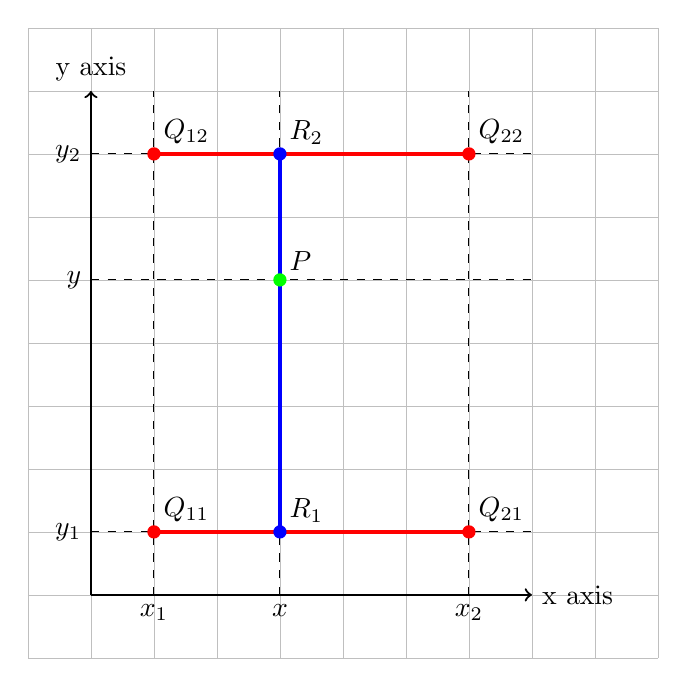
\begin{tikzpicture}[scale=0.8]

        % Grid
        \draw[step=1cm,gray!50,very thin] (-1,-1) grid (9,9);

        % Arrow
        \draw[thick,->] (0,0) -- (7,0) node[anchor=west] {x axis};
        \draw[thick,->] (0,0) -- (0,8) node[anchor=south] {y axis};

        % Dashed lines
        \draw[dashed] (1,0) -- (1,8) node[pos=0, below] {$x_1$};
        \draw[dashed] (3,0) -- (3,8) node[pos=0, below] {$x$};
        \draw[dashed] (6,0) -- (6,8) node[pos=0, below] {$x_2$};
        \draw[dashed] (0,1) -- (7,1) node[pos=0, left] {$y_1$};
        \draw[dashed] (0,5) -- (7,5) node[pos=0, left] {$y$};
        \draw[dashed] (0,7) -- (7,7) node[pos=0, left] {$y_2$};
        \draw[red, line width=1.5pt] (1,1) -- (6,1);
        \draw[red, line width=1.5pt] (1,7) -- (6,7);
        \draw[blue, line width=1.5pt] (3,1) -- (3,7);

        % Points
        \coordinate (Q11) at (1,1);
        \coordinate (Q12) at (1,7);
        \coordinate (Q21) at (6,1);
        \coordinate (Q22) at (6,7);
        \coordinate (R1) at (3,1);
        \coordinate (R2) at (3,7);
        \coordinate (P) at (3,5);

        % Labels
        \node[above right] at (Q11) {$Q_{11}$};
        \node[above right] at (Q12) {$Q_{12}$};
        \node[above right] at (Q21) {$Q_{21}$};
        \node[above right] at (Q22) {$Q_{22}$};
        \node[above right] at (R1) {$R_1$};
        \node[above right] at (R2) {$R_2$};
        \node[above right] at (P) {$P$};

        % Point styles
        \fill[red] (Q11) circle (3pt);
        \fill[red] (Q12) circle (3pt);
        \fill[red] (Q21) circle (3pt);
        \fill[red] (Q22) circle (3pt);
        \fill[blue] (R1) circle (3pt);
        \fill[blue] (R2) circle (3pt);
        \fill[green] (P) circle (3pt);

    \end{tikzpicture}
    \caption{Interpolation diagram.}
    \label{fig:interpolation}
\end{figure}

In the context of determining the value of an unknown function $f$ at a given coordinate $(x, y)$. Assuming we have knowledge of $f$ at four specified points: $Q_{11}=(x_1, y_1), Q_{12}=(x_1, y_2), Q_{21}=(x_2, y_1)$, and $Q_{22} = (x_2, y_2)$.

By performing linear interpolation in the x-direction, this yields

\begin{align*}
    f(x,y_{1})={\frac{x_{2}-x}{x_{2}-x_{1}}}f(Q_{11})+{\frac{x-x_{1}}{x_{2}-x_{1}}}f(Q_{21}) \\
    f(x,y_{2})={\frac{x_{2}-x}{x_{2}-x_{1}}}f(Q_{12})+{\frac{x-x_{1}}{x_{2}-x_{1}}}f(Q_{22})
\end{align*}

Then proceed by interpolating in the y-direction to obtain the desired estimate formula.

\begin{align*}
    f(x,y)= & {\frac {y_{2}-y}{y_{2}-y_{1}}}f(x,y_{1})+{\frac {y-y_{1}}{y_{2}-y_{1}}}f(x,y_{2})                                                                                                                                                                     \\
    =       & {\frac {y_{2}-y}{y_{2}-y_{1}}}\left({\frac {x_{2}-x}{x_{2}-x_{1}}}f(Q_{11})+{\frac {x-x_{1}}{x_{2}-x_{1}}}f(Q_{21})\right)+{\frac {y-y_{1}}{y_{2}-y_{1}}}\left({\frac {x_{2}-x}{x_{2}-x_{1}}}f(Q_{12})+{\frac {x-x_{1}}{x_{2}-x_{1}}}f(Q_{22})\right) \\
    =       & {\frac {1}{(x_{2}-x_{1})(y_{2}-y_{1})}}\bigl(f(Q_{11})(x_{2}-x)(y_{2}-y)+f(Q_{21})(x-x_{1})(y_{2}-y)                                                                                                                                                  \\
            & \quad \quad+f(Q_{12})(x_{2}-x)(y-y_{1})+f(Q_{22})(x-x_{1})(y-y_{1})\bigr)                                                                                                                                                                             \\
    =       & {\frac {1}{(x_{2}-x_{1})(y_{2}-y_{1})}}{\begin{bmatrix}x_{2}-x&x-x_{1}\end{bmatrix}}{\begin{bmatrix}f(Q_{11})&f(Q_{12})\\f(Q_{21})&f(Q_{22})\end{bmatrix}}{\begin{bmatrix}y_{2}-y\\y-y_{1}\end{bmatrix}}\text{, where}(x_2-x_1)(y_2-y_1)=1            \\
    =       & {\begin{bmatrix}x_{2}-x&x-x_{1}\end{bmatrix}}{\begin{bmatrix}f(Q_{11})&f(Q_{12})\\f(Q_{21})&f(Q_{22})\end{bmatrix}}{\begin{bmatrix}y_{2}-y\\y-y_{1}\end{bmatrix}}
\end{align*}

As a result, by computing $f(x+dx, y+dy)=(1-dx)(1-dy)f(x,y)+x(1-y)f(x+1,y)+(1-dx)yf(x,y+1) +xyf(x+1,y+1)$ can get the result directly.

\section{Part 3.}
\subsection{Paste the 2 warped images and the link you find}

After scanning the QR code, you'll get the URL \href{https://qrgo.page.link/jc2Y9}{https://qrgo.page.link/jc2Y9}, which subsequently redirects to the \href{http://media.ee.ntu.edu.tw/courses/cv/21S/}{Computer Vision: from Recognition to Geometry} website.

\begin{figure}[H]
    \centering
    \begin{minipage}{.4\textwidth}
        \centering
        \includegraphics[width=.5\linewidth]{./src/output3_1.png}
        \captionof{figure}{First warped image.}
        \label{fig:output3_1}
    \end{minipage}%
    \begin{minipage}{.4\textwidth}
        \centering
        \includegraphics[width=.5\linewidth]{./src/output3_2.png}
        \captionof{figure}{Second warped image.}
        \label{fig:output3_2}
    \end{minipage}
\end{figure}

\subsection{Discuss the difference between 2 source images, are the warped results the same or different?}

\begin{figure}[H]
    \centering
    \includegraphics[width=0.5\textwidth]{./resource/BL_secret1.png}
    \caption{The first source image.}
    \label{fig:BL_secret1}
\end{figure}

\begin{figure}[H]
    \centering
    \includegraphics[width=0.5\textwidth]{./resource/BL_secret2.png}
    \caption{The second source canvas.}
    \label{fig:BL_secret2}
\end{figure}

Looking at the two original images, it is obvious that the QR code on the roof in the first image (Figure \ref{fig:BL_secret1}) seems to be more square-shaped and free from distortion, whereas the QR code on the roof in the second image (Figure \ref{fig:BL_secret2}) exhibits bending and distortion. As a consequence, the QR code (Figure \ref{fig:output3_1}) produced from the first image displays a sharper image, whereas the QR code (Figure \ref{fig:output3_1}) derived from the second image seems blurrier. Nonetheless, both QR codes can be scanned to access the same website successfully.

\subsection{If the results are the same, explain why. If the results are different, explain why?}
The results are the same. A blurred QR code can be successfully scanned due to Reed-Solomon error correction. This technique adds redundancy to the QR code's data, allowing for error detection and correction. Even when the code is damaged or obscured, the algorithm reconstructs the original data, ensuring successful scanning. Thus, the combination of error detection, correction, and data reconstruction ensures that even a blurred QR code can be effectively interpreted by scanning devices.

\section{Part 4.}
\subsection{Paste your stitched panorama}

\begin{figure}[H]
    \centering
    \includegraphics[width=0.8\textwidth]{./src/output4.png}
    \caption{The stitched panorama.}
    \label{fig:part4}
\end{figure}

\subsection{Can all consecutive images be stitched into a panorama?}
The consecutive images provided by TA can appropriately be stitched into a panorama as needed, although it's common for not all consecutive images to be suitable for panorama stitching.

\subsection{If yes, explain your reason. If not, explain under what conditions will result in a failure?}
It is obvious that if the number of detected features in the overlapping area between the two consecutive image frames is not sufficient, stitching failure will occur during the transformation, and this might cause misalignment or incomplete merging. Moreover, A simple concatenation of images with overlapping areas to form a panoramic image results in visible seams due to variations in the angle viewpoint of the camera and scene illumination, along with the spatial position errors of the images. As a result, the success or failure depends on the qualities of consecutive image frames.

% BibTex
% \bibliographystyle{ieeetr}
% \bibliography{reference}

\end{document}